\chapter{筵席的邀約（19:1-19:21）}

啟示錄十九章把我們帶到兩個截然不同的「筵席」面前。一方面，是羔羊的婚筵\idx{10}{羔羊的婚筵}：「凡被請赴羔羊\idx{10}{羔羊}之婚筵的有福了。」羔羊的新婦\idx{13}{新婦}已經預備好了，天上充滿讚美。這是羔羊與祂子民的筵席，象徵救恩、喜樂與永恆的團契。

另一方面，卻有「神的大筵席\idx{10}{神的大筵席}」。這個筵席，飛鳥被召聚，是給飛鳥吃盡那些敵對神之人的肉。

隨後，騎白馬\idx{05}{白馬}的基督顯現。祂名為「誠信真實」，按著公義審判\idx{15}{審判}、爭戰，擊潰獸和假先知\idx{11}{假先知}。這位曾經被世人拒絕、逼迫\idx{13}{逼迫}的基督，顯明祂的榮耀\idx{14}{榮耀}，一切敵對神的勢力，在祂面前都不能站立。

今天，羔羊仍然發出祂的邀請。願我們以信心接受祂的恩典\idx{10}{恩典}，忠心跟隨祂，預備自己迎接那位即將再來的君王。

\section{羔羊之婚筵}

\begin{ScriptureBox2}{數一數「哈利路亞」出現了幾次。群眾為什麼讚美神？新婦蒙恩得穿什麼？}

\item[19:1] 此後、我聽見好像群眾在天上大聲說、哈利路亞、〔就是要讚美耶和華的意思〕救恩、榮耀、權能、都屬乎我們的　神．

\item[19:2] 他的判斷是真實公義的．因他判斷了那用淫行敗壞世界的大淫婦、並且向淫婦討流僕人血的罪、給他們伸冤。

\item[19:3] 又說、哈利路亞。燒淫婦的煙往上冒、直到永永遠遠。

\item[19:4] 那二十四位長老與四活物、就俯伏敬拜坐寶座的　神、說、阿們、哈利路亞。

\item[19:5] 有聲音從寶座出來說、　神的眾僕人哪、凡敬畏他的、無論大小、都要讚美我們的　神。

\item[19:6] 我聽見好像群眾的聲音、眾水的聲音、大雷的聲音、說、哈利路亞．因為主我們的　神、全能者、作王了。

\item[19:7] 我們要歡喜快樂、將榮耀歸給他．因為羔羊婚娶的時候到了、新婦也自己預備好了。

\item[19:8] 就蒙恩得穿光明潔白的細麻衣、這細麻衣就是聖徒所行的義。

\item[19:9] 天使吩咐我說、你要寫上、凡被請赴\textbf{羔羊之婚筵}的有福了。又對我說、這是　神真實的話。

\item[19:10] 我就俯伏在他腳前要拜他。他說、千萬不可．我和你並你那些為耶穌作見證的弟兄同是作僕人的．你要敬拜　神．因為預言中的靈意、乃是為耶穌作見證。

\end{ScriptureBox2}

天上的群眾讚美神，因為神的判斷是真實公義的。神公義完全彰顯，所以他們的讚美。這裡包含了6:10殉道\idx{10}{殉道}者。他們曾經問：「聖潔真實的主啊，你不審判\idx{15}{審判}住在地上的人，給我們伸流血的冤，要等到幾時呢？」

\begin{ReaderQuestion}
19:9說「凡被請赴羔羊之婚筵的有福了」。如果我們真正相信自己是被邀請赴羔羊婚筵的人，今天的生活態度應該有什麼不同？
\end{ReaderQuestion}

\section{騎白馬的基督：萬王之王}


\begin{figure}[htbp]
    \centering
    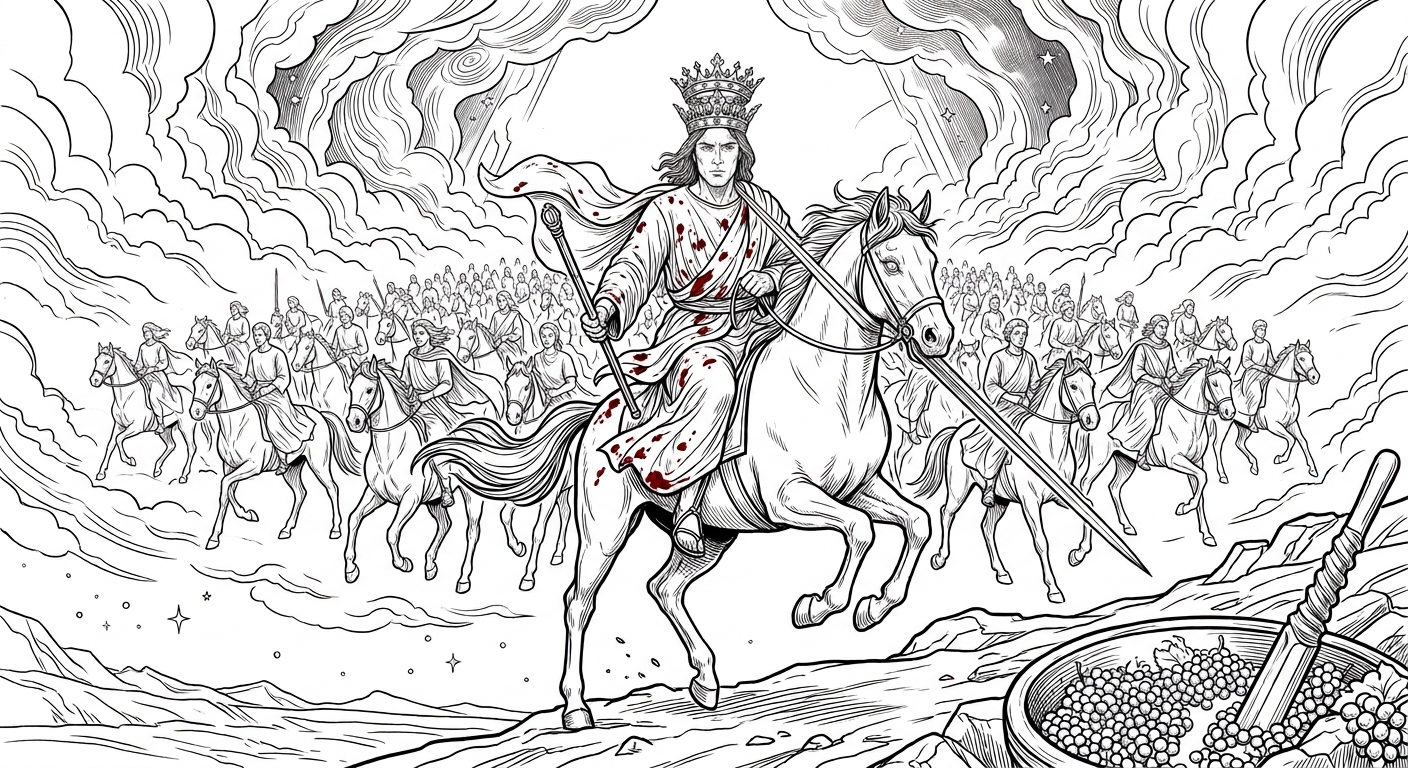
\includegraphics[
    width=1\textwidth, 
    trim=0 0 0 0, 
    clip]{images/christ_blood_white_horse.jpg}
    %\caption{}
    %\label{}
\end{figure}


\begin{ScriptureBox2}{圈出騎白馬者的每一個名字和稱號。祂穿著什麼？從祂口中出來的是什麼？}

\item[19:11] 我觀看、見天開了．有一匹白馬．騎在馬上的、稱為誠信真實．他審判爭戰都按著公義。

\item[19:12] 他的眼睛如火焰、他頭上戴著許多冠冕．又有寫著的名字、除了他自己沒有人知道。

\item[19:13] 他穿著濺了血的衣服．他的名稱為　神之道。

\item[19:14] 在天上的眾軍、騎著白馬、穿著細麻衣、又白又潔、跟隨他。

\item[19:15] 有利劍從他口中出來、可以擊殺列國．他必用鐵杖轄管他們．〔轄管原文作牧〕並要踹全能　神烈怒的酒醡。

\item[19:16] 在他衣服和大腿上、有名寫著說、萬王之王、萬主之主。

\end{ScriptureBox2}

這裡有一匹白馬\idx{05}{白馬}以及騎在白馬上的基督。此白馬與騎士不是啟示錄第四章的白馬。這裡我們更可以認識基督的榮耀\idx{14}{榮耀}形象。祂的衣服濺了血，因為他曾用祂的血救贖\idx{11}{救贖}我們。祂是\textit{萬王之王、萬主之主。}

\begin{ReaderQuestion}
19:11–16用了哪些名稱或圖像描寫基督？「誠信真實」、「神之道」、「萬王之王、萬主之主」各自帶給你什麼提醒？
\end{ReaderQuestion}

\section{神的大筵席}

\begin{ScriptureBox2}{誰被召聚來赴神的大筵席？獸和假先知遭遇了什麼？其餘的人又怎樣？}

\item[19:17] 我又看見一位天使站在日頭中、向天空所飛的鳥、大聲喊著說、你們聚集來赴　\textbf{神的大筵席．}

\item[19:18] 可以喫君王與將軍的肉、壯士與馬和騎馬者的肉、並一切自主的為奴的、以及大小人民的肉。

\item[19:19] 我看見那獸、和地上的君王、並他們的眾軍、都聚集、要與騎白馬的、並他的軍兵爭戰。

\item[19:20] 那獸被擒拿、那在獸面前曾行奇事、迷惑受獸印記、和拜獸像之人的假先知、也與獸同被擒拿．他們兩個就活活的被扔在燒著硫磺的火湖裡．

\item[19:21] 其餘的被騎白馬者口中出來的劍殺了．飛鳥都喫飽了他們的肉。

\end{ScriptureBox2}

啟示錄將兩個「筵席」放在同一章中，「神的大筵席\idx{10}{神的大筵席}」與前面的「羔羊\idx{10}{羔羊}婚筵」形成強烈對比。羔羊的婚筵\idx{10}{羔羊的婚筵}是屬於基督和祂子民的救恩與喜樂；神的大筵席則象徵敵對神之勢力所面對的最後審判\idx{15}{審判}。

\begin{ReaderQuestion}
如果你在患難、誘惑或不確定的環境中讀19章，哪一個信息最能堅固你的信心：神的審判真實公義、羔羊婚筵、基督是萬王之王，或羔羊最終得勝？為什麼？
\end{ReaderQuestion}
